\documentclass[12pt]{article}

\usepackage{sbc-template}
\usepackage{CJKutf8}

\usepackage{graphicx,    url}

\usepackage[brazil]{babel}   
%\usepackage[latin1]{inputenc}  
\usepackage[utf8]{inputenc}  
% UTF-8 encoding is recommended by ShareLaTex
\usepackage{cases}
\usepackage{amsfonts}
\usepackage{listings}
\usepackage[linesnumbered,algoruled,boxed,lined]{algorithm2e}
\sloppy
\usepackage{float}



\begin{document} 
\begin{CJK*}{UTF8}{gbsn}


\section{背景介绍}




近年来,     由于电脑硬件计算速度的极大提高以及并行计算方法的不断完善,     机器学习在各个领域都获得了很大的成绩. 在医疗领域的各个方面,     包括计算机辅助诊断(computer-aided diagnosis),图像
分割(image segmentation),图像配准(image registration),图像融合(image fusion),图像引导疗法(image-guided therapy),图像注释(image annotation)和图像数据库检索(image database retrieval),     机器学习的方法都可以加以运用,     帮助医生作出初步诊断以及改善患者的医疗保健条件.目前已经取得的一些成果包括:乳腺癌的早期检测\cite{tang2009computer},     肺部疾病分类 \cite{raghunath2013landscaping},     \cite{sluimer2006computer},     等等. \\
\\
深度学习方法是机器学习当中一组重要的算法,     它可以通过多层网络的学习和提取抽象信息来帮助我们理解和解释医疗数据. 机算机神经网络算法最初从生物学获得灵感,     更准确的说是从人类大脑的神经网络结构中得到的启发\cite{krenker2011introduction}, 逐步发展成为如今从理论和实现都相对完善的学科. 我们首先通过解释神经网络的一些基本概念,比如神经元,权重和激活函数来模拟非线性数据. 之后描述了如何设计和训练神经网络,     从而达到我们通过CT图像来寻找缺血性卒中患者的梗死核心和半暗带识别的目的. 基本框架如下所述:

\section{神经网络框架}

\subsection{基本概念}

神经网络由彼此链接的单个神经元(neurons) 组成. 神经元是神经网络架构的基石,    同时每一个单独的神经元也可以看做是一个简单的分类模型. 图\ref{fig:fig1}显示了一个神经元的样例,     一个神经元使用使用一组特征$x_i$作为输入,     对它们进行线性组合并且加上一定的偏移量(bias)作为输出. 公式(\ref{eq:netron})给出了它的数学定义.其中参数$w_i$ 代表了每一个特征的权重,     参数$b$ 代表了偏移量,     函数$f(.)$ 代表了非线性激活函数(nonlinear activation function). 
\begin{equation} \label{eq:netron}
output = f(\sum_{i=1}^3 w_ix_i+b)
\end{equation}

\begin{figure}[ht]
\centering
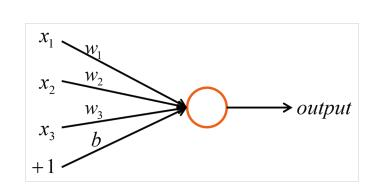
\includegraphics[width=.5\textwidth]{figure1.jpg}
\caption{神经元示例}
\label{fig:fig1}
\end{figure}
\\
\\
在计算过程当中,     每一个输入值 $x_i$ 都乘以了它对应的权重 $w_i$. 然后对于加权后的输入值以及偏移量$b_i$进行求和. 求和之后的结果输入一个非线性激活函数$f(.)$ 从而得到一个神经元的最终结果. 比较常见的激活函数有: 逻辑S函数(Logistic Sigmoid Function),     双曲正切函数(Hyperbolic Tangent Function),    线性整流函数(Rectified Linear Unit,     ReLU)以及带泄露线性整流函数(Leaky ReLU). 它们的具体样式在图2中给出了示例.


\begin{figure}[H]
\centering
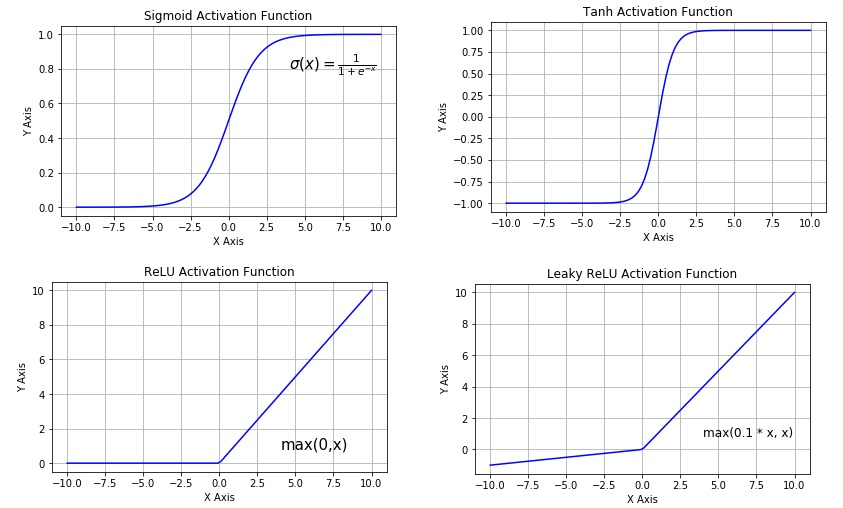
\includegraphics[width=1\textwidth]{activation.jpg}
\caption{激活函数示例: 左上代表了逻辑S函数(Logistic Sigmoid Function),    右上代表了双曲正切函数(Hyperbolic Tangent Function),    左下代表了线性整流函数(Rectified Linear Unit,    ReLU)以及右下代表了带泄露线性整流函数(Leaky ReLU)}
\label{fig:fig1}
\end{figure}

公式(2) - (5) 给出了它们的数学定义.\\
\\
逻辑S函数(Logistic Sigmoid Function):
\begin{equation} \label{eq:sigmoid}
\end{equation}
双曲正切函数(Hyperbolic Tangent Function):
\begin{equation} \label{eq:tanh}
f(x) = \frac{e^x-e^{-x}}{e^x+e^{-x}}
\end{equation}
线性整流函数(Rectified Linear Unit,    ReLU)
\begin{equation} \label{eq:relu}
f(x) = max(0,   x)
\end{equation}
带泄露线性整流函数(Leaky ReLU)
\begin{equation}
f(x) = 
\left\{
\begin{array}{rl}
x&if\ x > 0\\
0.01x&otherwise
\end{array}
\right.
\end{equation}

\subsection{多层感知器}

神经网络模型由多个连接在一起的神经元组成.正如在神经元的简单例子(图1)中可以看到的那样, 一个神经元的输出可以是另一个神经元的输入. 图3给出了一个小型前馈神经元的例子. 这样的网络也被称为多层感知器,其中神经元被分组为各层
并且完全连接到下一层(每一层的神经元与下一层的神经元完全连接),并且连接不会形成任何闭合的有向循环.输入也用圆圈表示(图中用蓝色表示),用“+1”标记的圆圈对应于之前提到的偏移量。偏移量没有输入,因为它们总是输出+1.最左边的图层称为输入图层,最右边的图层称为输出图层。中间的图层表示为隐藏层,因为它的值在训练集中没有被观察到.神经元(用橙色圆圈表示)也可以被看做是一个单独的计算单位(unit). 

\begin{figure}[H]
\centering
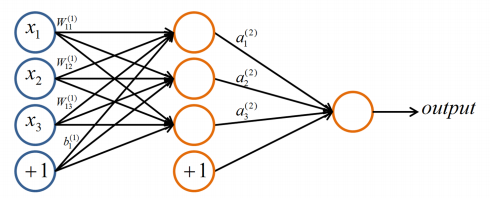
\includegraphics[width=1\textwidth]{forward.png}
\caption{多层感知器模型示例:多层感知器模型也可以被称作前向神经网络,用蓝色圆圈表示输入层,橙色圆圈表示神经元以及最终的输出层. 权重用每一层神经元与神经元之间的对应边来表示, 偏移量(bias)通过值为+1的结点来表示. $a_i^{(l)}$代表了第$i$层的第$l$个节点, 最终输出一个分类结果}
\label{fig:fig1}
\end{figure}
\\
图3中显示了多层感知器的一个简单结构,其中, 第i层标记为$L_i$,    总共的层数$n_L=3$. 第一层$L_1$作为输入层, 代表的是我们的训练样本. 第二层也可以称为隐藏层,记为$L_2$,    第三层是$L_3$,   也代表我们的输出层,通常会给出一个分类的结果或者概率.
模型的参数是$(W,   B)=(W^{(1)},   b^{(1)},   W^{(2)},   b^{(2)})$,    这里的$b_i^{(l)}$表示第i层对应结点的偏移量, $W_{ij}^{(l)}$ 第l层的第i个结点到第$l+1$层的第j个结点的权重.由于我们只有三层网络,所以$W^{(1)}\in \mathbb{R}^{3\times 3$,    $W^{(2)}\in \mathbb{R}^{1\times 3}$,    $b^{(1)}\in \mathbb{R}^3$ and $b^{(2)}\in \mathbb{R}^1$. 每一层的激活函数结果计算如下:

\begin{equation}
a_1^{(2)}=f(W_{11}^{(1)}x_1+W_{12}^{(1)}x_2+W_{13}^{(1)}x_3+b_1^{(1)})
\end{equation}
\begin{equation}
a_2^{(2)}=f(W_{21}^{(1)}x_1+W_{22}^{(1)}x_1+W_{23}^{(1)}x_1+b_2^{(1)})
\end{equation}
\begin{equation}
a_3^{(2)}=f(W_{31}^{(1)}x_1+W_{32}^{(1)}x_1+W_{33}^{(1)}x_1+b_3^{(1)})
\end{equation}
这个$a_i^l$ 表示的是第l层第i个单位的激活函数, $f(.)$代表了非线性激活函数的表达式.第l层激活函数的的结果作为第l+1层神经元的输入, 最后一层输出层的计算公式如下:

\begin{equation}
output = a_1^{(3)}= \sigma(W_{11}^{(2)}a_1^{(2)}+W_{12}^{(2)}a_2^{(2)}+W_{13}^{(2)}a_3^{(2)}+b_1^{(2)}
\end{equation}
这里的$\sigma$ 代表了输出层的激活函数,一般我们采用逻辑S函数(Logistic Sigmoid Function),    值得注意的是输出层的激活函数与隐藏层的激活函数通常不同,因为在输出层我们一般需要分类的结果,所以采用Sigmoid 函数来返回一个概率的结果.这样的每层逐步计算的过程通常成为前向繁衍(forward propagation) . 我们通常熟知的深度学习一般就是通过这样的过程不断增加新的隐藏层来得到的.同时我们必须也要指定每一层的节点个数.另外,我们的输出层不仅限于二进制分布,同样适用于多类别的分类问题, 区别就是输出层的结果$y$从二维$\{0,   1\}$分布,变为了一个n维${0,   1,   ...,   n}$ 的目标输出值.

\subsection{反向传播}

上一节我们介绍了前向神经网络的架构,对于神经网络来说如何调整参数使得最终的分类误差达到最小是我们的主要目标.目前一般采用反向传播梯度下降的方法(Back Propagation Gradient Decent)来最优化参数. 我们假设整个前馈网络的输出结果为$O_k$,     神经元激活函数的输出结果为$\sigma^i(k),    i =1 ,    2,    ...,    n$.在每一次反向传播的时候更新权重$W$:
\begin{equation}
    W(k+1) = W(k) -\lambda \frac{\partial E}{\partial w}
\end{equation}

这里输出层的分类误差为: 
\begin{equation}
    E=\frac{1}{2} \sum_{k=1}^{n}(t_k-O_k)^2
\end{equation}

其中$t_k$为第k个样本的真实类别.

对于每一层的梯度推导如下:\\
输出层:
\begin{equation}
 \frac{\partial E}{\partial w_{jk}}=-\sum_k(t_k-O_k)\frac{\patial O_k}{\partial w_{jk}}
\end{equation}
隐层:
\begin{equation}
 \frac{\partial E}{\partial w_{ij}}=-\sum_k(t_k-O_k)\frac{\patial O_k}{\partial w_{ij}}
\end{equation}
线性神经元:
\begin{equation}
 \frac{\partial E}{\partial w_{l}}=-\sum_k(t_k-O_k)\frac{\patial O_k}{\partial w_{l}}=-\sum_k(t_k-O_k)\frac{\patial O_k}{\partial \sigma_k}\frac{\partial \sigma_k}{\partial w_l}
\end{equation}
算法1给出了反向传播过程的伪代码. 我们可以更加直观的了解神经网络的更新过程.

\begin{algorithm}[H]
\SetKwData{Left}{left}
\SetKwData{This}{this}
\SetKwData{Up}{up}
\SetKwFunction{Union}{Union}
\SetKwFunction{FindCompress}{FindCompress}
\SetKwInOut{Input}{input}
\SetKwInOut{Output}{output}
$\textbf{输入:}$\\
\ \ \ 数据样本$(\textbf{x,y})$,权重向量$\textbf{w}$, 层次网络$\textbf(V,E)$, 其中$\textbf{V}$代表了网络中的节点, $\textbf{E}$代表了网络中的边\\
\ \ \ 激活函数 $\sigma: \mathbb{R}\rightarrow \mathbb{R}$\\
$\textbf{初始化:}$\\ 
\ \ \ 初始化网络结构中的每一层节点向量$\textbf{V}_0,...,\textbf{V}_T$, 其中$\textbf{V}_t=\{v_{t,1},..., v_{t,k_t}\}$\\\\
\ \ \ 初始化第t层到第t+1层($(v_{t,j}, v_{t+1,i})$)的权重 $W_t,i,j$, 其中如果 $(v_{t,j}, v_{t+1,i}}\notin E)$, 那么我们设置$W_{t,i,j}=0$\\
$\textbf{前向过程:}$\\
\ \ 设置$\textbf{O}_0=\textbf{x}$\\
\ \ \For{$t= 1,..., T$}{
\For{$i = 1, ..., k_t$}{
设置 $a_{t,i}=\sum_{j=1}^{k_{t-1}}W_{t-1,i,j} O_{t-1,j}$\\
设置 $O_{t,i}= \sigma(a_{t,i})$\\
}
}
$\textbf{反向过程:}$\\
\ \ \ 设置$\delta_T=\textbf{O}_T-\textbf{y}$\\
\ \ \For{$t=T-1,T-2,...,1$}{
\For{$i = 1, ..., k_t$}{
\ \ \ 设置 $\delta_{t,i}=\sum_{j=1}^{k_{t+1}} W_{t,i,j}\delta_{t+1,j} \sigma'(a_{t+1,j})$
}
}
$\textbf{输出:}$\\
\ \ 对于每一条边$(v_{t-1,j},v_{t,i})\in E$ \\
\ \ \ \ 输出偏导数 $\delta_{t,i} \sigma'(a_{t,i}) O_{t-1,j}$

\caption{反向传播过程}\label{alg:backpropagation}
\end{algorithm}


\section {CT图像半暗带诊断模型}
\subsection{基本框架}
我们本次研究拟利用深度神经网络来帮助医生对于脑卒中患者缺血半暗带区域进行预判断.主要目的是希望能够减少人为判断带来的误差, 同时可以为医生初诊提供依据并且节约医生人工诊断的时间.图4给出了脑卒中患者CT图像的示例,上图患者在一个时刻的脑部CT原始图像,下图是同一时刻患者脑部CT图像对应的半暗带区域,其中绿色部分是具体的缺血半暗带区域.我们希望通过运用深度神经网络模型, 当输入患者的原始CT图像之后,通过模型能够准确指出半暗带区域. 
\begin{figure}[H]
\centering
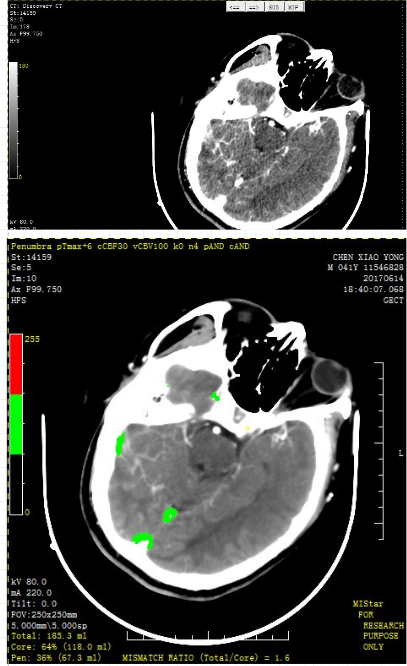
\includegraphics[width=0.6\textwidth]{ct_chart.png}
\caption{卒中患者脑部CT示例:上图为卒中患者脑部CT原始图像,下图为患者的脑缺血半暗带区域,其中绿色的部分代表了真实发生的半暗带区域}
\label{fig:fig1}
\end{figure}

卷积神经网络模型(CNN)主要包含三种网络层: 卷积层 (Convolutions) , 采样层(Subsampling)和全连接层(fully connected). 我们首先从原始的图像中截取部分图像组成训练样本, 在训练样本中, 我们根据原始图像和标注半暗带区域的图像对于截取的图像进行分类, 如图5所示,上半部分图像截取的范围涉及到了脑缺血半暗带区域,因此我们标注为1, 即该部分图像成阳性, 下半部分的图像截取的范围没有涉及到脑缺血的区域, 因此我们标注为0, 即该部分图像呈阴性. 图6给出了模型的简要结构, 包含了两个卷积层, 两个采样层和一个全连接层(即最终的输出层).每一层的输入由上一层的输出得到. 

\begin{figure}[H]
\centering
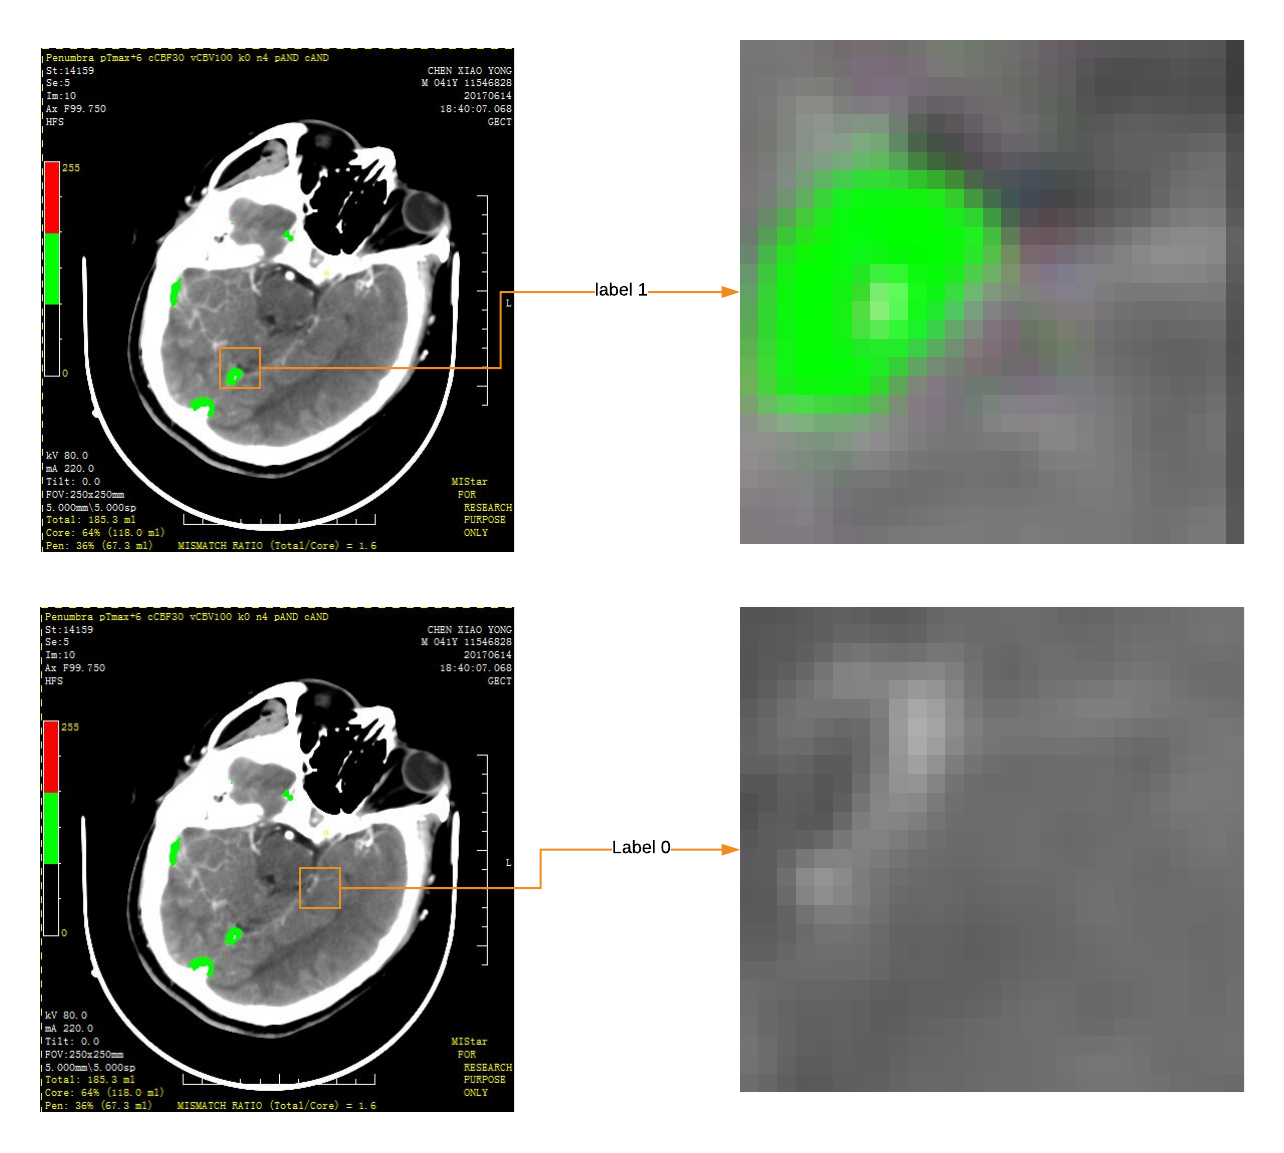
\includegraphics[width=0.9\textwidth]{slice.png}
\caption{脑CT图像截取示意图: 原始CT图像的大小为422 $\times$ 733, 我们从中抽取相同长度和宽度的小部分作为训练样本, 对于每一小块,根据实际的图像情况进行分类, 上半部分图像截取的范围涉及到了脑缺血半暗带区域,因此我们标注为1, 即该部分图像成阳性, 下半部分的图像截取的范围没有涉及到脑缺血的区域, 因此我们标注为0, 即该部分图像呈阴性.}
\label{fig:fig1}
\end{figure}


\begin{figure}[H]
\centering
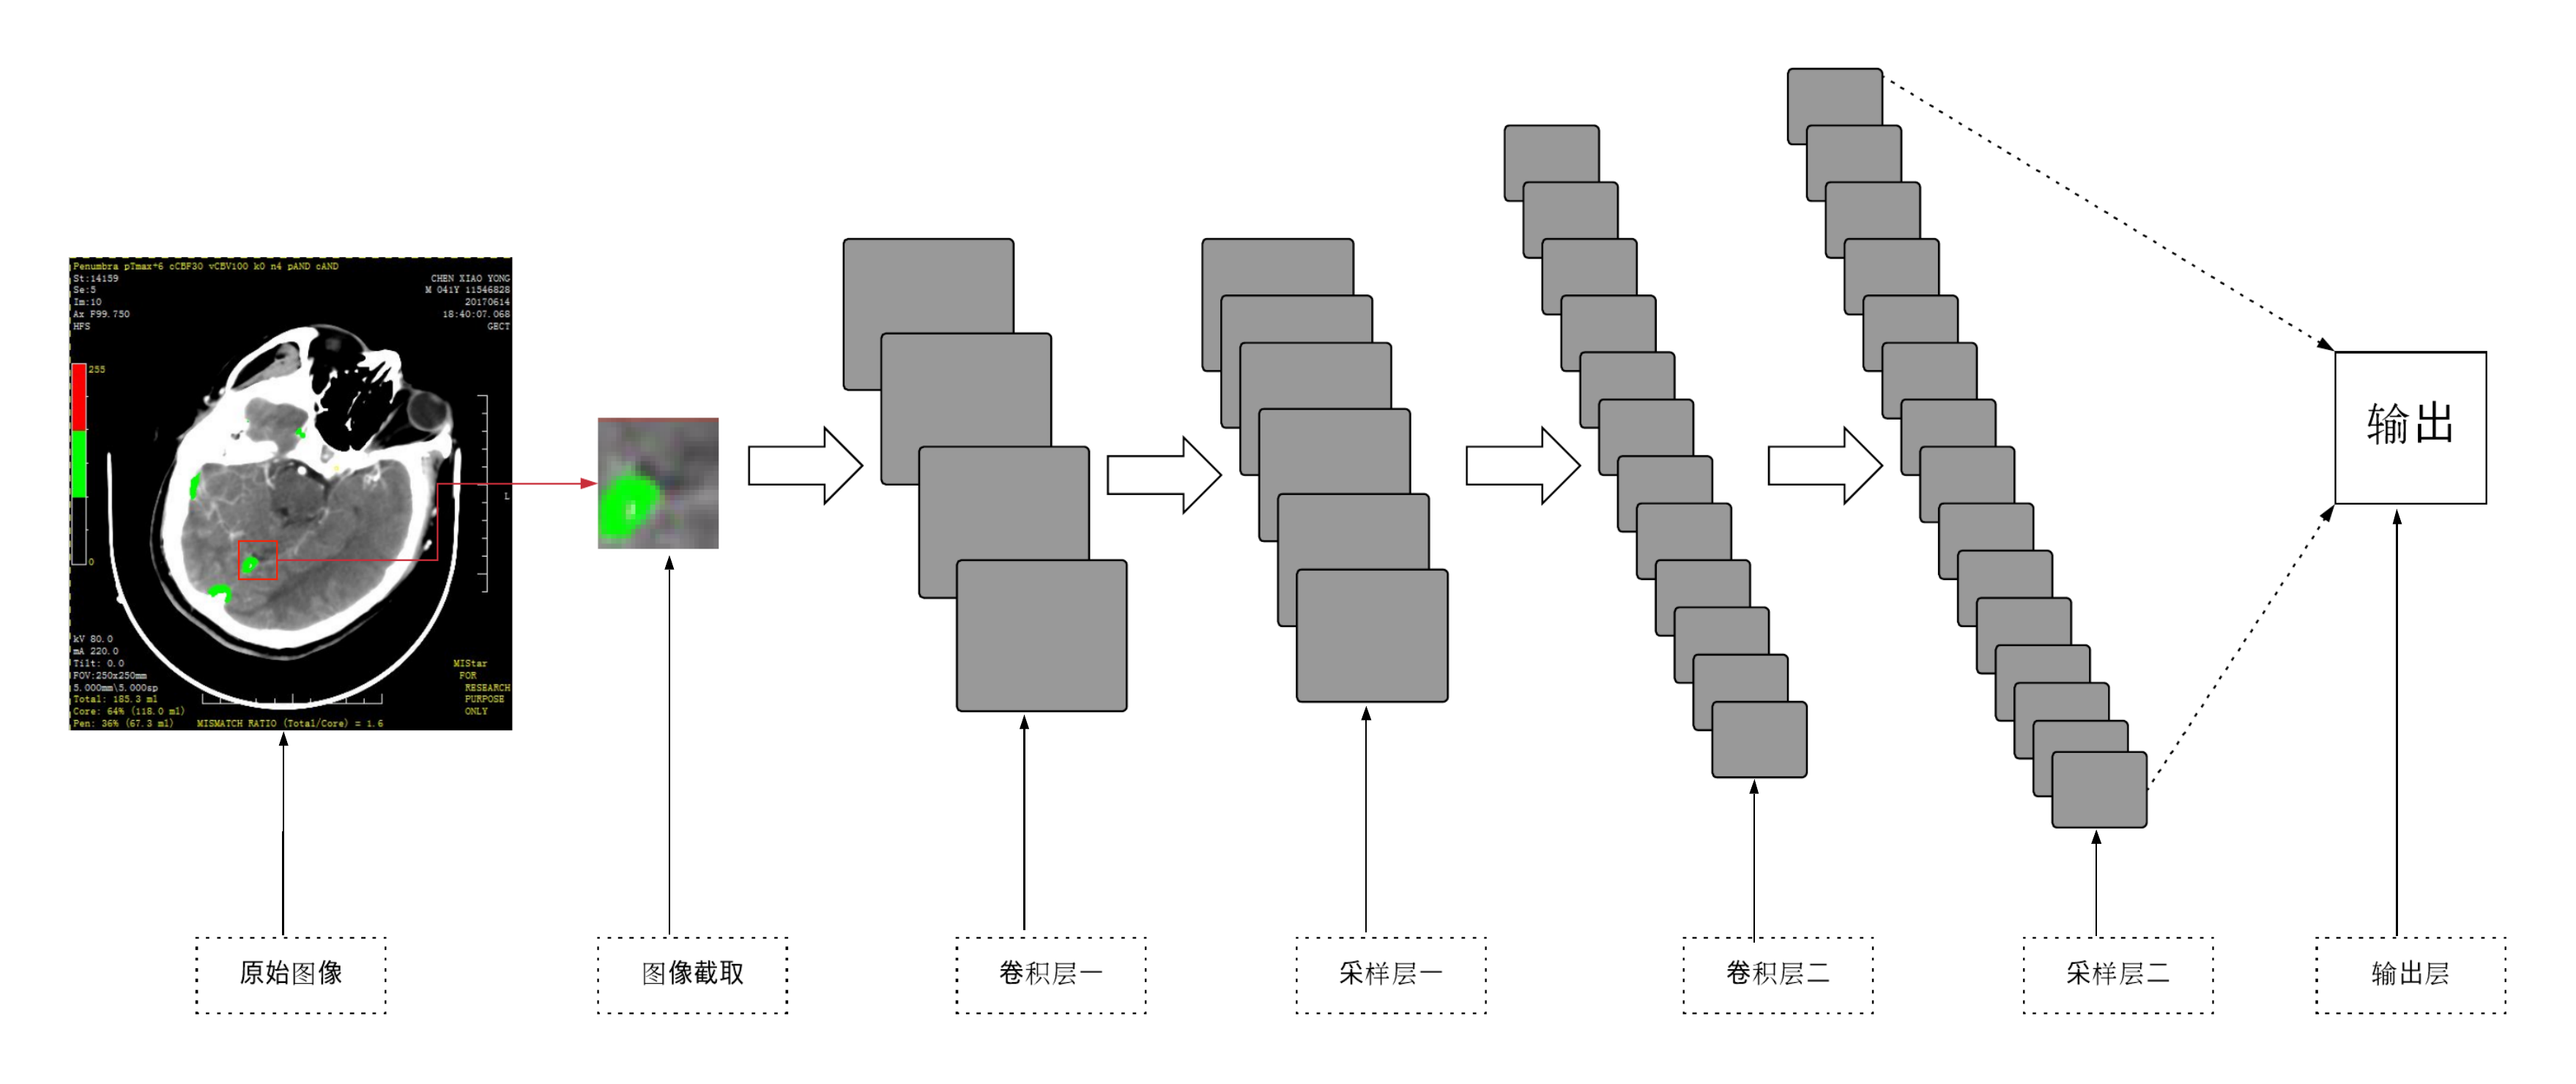
\includegraphics[width=1\textwidth]{cnn_struc2.png}
\caption{深度卷积神经网络结构示意图: 包含了两个卷积层, 两个采样层和一个全连接层(即最终的输出层)}
\label{fig:fig1}
\end{figure}

\subsection{模型实现}

对于深度学习来说, 目前常用的框架是Google 公司开发的Tensorflow系统, 我们的研究主要采用Keras软件包配合OpenCV等图像处理系统. Keras是一个基于Theano和Tensorflow的深度学习Python软件包, 它的开发旨在尽可能快速和便利地搭建深度学习模型. Python 2.7或3.5上都可以运行Keras,并且它对于GPU和CPU可以实现无缝连接.我们之所以使用Keras, 主要是它具有以下的一些优势:
\begin{itemize}
    \item 模块化:模型可以被理解为一个序列或一个图从而使得深度学习模型当中的任何独立部分都可以被任意地组合.
\item 简洁性:keras只提供了能够实现结果的最简单的程序, 没有提供冗余的程序来增加可读性。
\item 可扩展性:Keras很容易添加新的框架和组件,方便研究人员试用和探索新想法。
\end{itemize}
下面提供了Keras深度学习模型的Python 程序示例.

\begin{lstlisting}[language=Python, caption=Keras example]
def getModel():
    model=Sequential()
    
    # CNN 1
    model.add(Conv2D(64, kernel_size=(3, 3),activation='relu', input_shape=(75, 75, 3)))
    model.add(MaxPooling2D(pool_size=(3, 3), strides=(2, 2)))
    model.add(Dropout(0.2))

    # CNN 2
    model.add(Conv2D(128, kernel_size=(3, 3), activation='relu' ))
    model.add(MaxPooling2D(pool_size=(2, 2), strides=(2, 2)))
    model.add(Dropout(0.2))

    # CNN 3
    model.add(Conv2D(128, kernel_size=(3, 3), activation='relu'))
    model.add(MaxPooling2D(pool_size=(2, 2), strides=(2, 2)))
    model.add(Dropout(0.2))

    #CNN 4
    model.add(Conv2D(64, kernel_size=(3, 3), activation='relu'))
    model.add(MaxPooling2D(pool_size=(2, 2), strides=(2, 2)))
    model.add(Dropout(0.2))

    model.add(Flatten())

    #Dense 1
    model.add(Dense(512, activation='relu'))
    model.add(Dropout(0.2))

    #Dense 2
    model.add(Dense(256, activation='relu'))
    model.add(Dropout(0.2))

    # Output 
    model.add(Dense(1, activation="sigmoid"))

    optimizer = Adam(lr=0.001, decay=0.0)
    model.compile(loss='binary_crossentropy', optimizer=optimizer, metrics=['accuracy'])
    
    return model
\end{lstlisting}
\subsection{数据增强}
一般来说, 深度学习模型应用于大型的训练集能够取得最显著的成果, 但在医疗领域当中, 并不总是能够获取足够的数据集, 一般有两种方法可以解决数据量较少的问题:迁移学习和微调现有图像. 由于医疗影像的特殊性, 迁移学习并不十分适合于应用在这个领域, 因此我们主要使用微调现有的数据来增加训练集样本.图7给出了原始图像微调的一个示例, 可以看出,通过数据增强的技术, 我们可以利用一张图像生成图中显示的100张图像, 每一张新生成的图像都可以作为一个新的训练样本. 我们使用的图像调整技术主要包括: 旋转(Rotation), 平移(transportation), 裁剪(Shear) 以及明亮度调节(Brightness).


\begin{figure}[H]
\centering
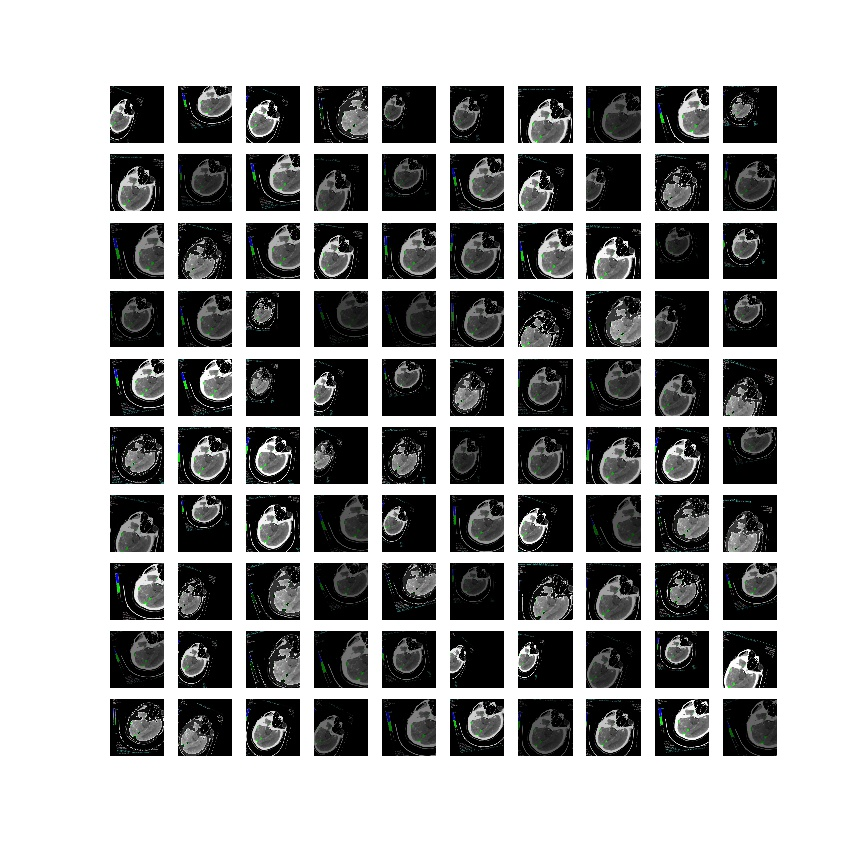
\includegraphics[width=1.2\textwidth]{augumentation.jpg}
\caption{医疗影像数据增强示例}
\label{fig:fig7}
\end{figure}

\section{合作者信息:}
张锦峰:佛罗里达州立大学统计系终身教授,    哈佛大学统计专业博士后,      
芝加哥伊利诺伊大学计算机专业硕士,    统计专业博士,     北京大学学士,     多年从事机器学习以及生物医疗方面研究.\\
个人主页:https://ani.stat.fsu.edu/~jinfeng/\\
\\
王剑: 佛罗里达州立大学金融数学博士,上海大学数学系硕士及本科. 主要从事机器学习在金融数据中应用等方面的研究课题.\\
个人主页:https://jianwang2018.github.io/jianwang.github.io/





\clearpage\end{CJK*}


\bibliographystyle{sbc}
\bibliography{sbc-template}

\end{document}
